\documentclass[11pt]{article}

\usepackage[margin=0.8in]{geometry}
\usepackage[T1]{fontenc}
\usepackage{lmodern}
\usepackage{booktabs}
\usepackage{graphicx}
\usepackage{hyperref}
\usepackage{pgfplots}
\pgfplotsset{compat=1.18}
\setlength{\emergencystretch}{2em}

\title{Microarchitectural Characterization of Dynamic Language Runtimes\\
\large Checkpoint I: Baseline Cache, Branch, and Stall Measurements}
\author{Y Tagore Ravindra Sree}
\date{\today}

\begin{document}
\maketitle

\begin{abstract}
This report compares five small workloads in Python and Java. They test
different memory and branch patterns. PIN captures each program's instructions,
and ChampSim replays them. Java pointer chasing stood out in these results.
Python's five workloads looked more alike. These are simulator results, not
program run times on a real processor.
\end{abstract}

\section{Why this question?}
Dynamic languages do more than the operations written in source code.
Interpreters and runtimes also run instructions. These extra instructions can
affect memory access and branches. I wanted to see which workload patterns
stand out in Python and Java traces. This is an early comparison, not a
general ranking of the two languages.

\section{Workloads}
\begin{itemize}
  \item \textbf{Sequential}: scans a 65,536-element array or list.
  \item \textbf{BranchPredictable}: takes one branch outcome most of the time.
  \item \textbf{BranchUnpredictable}: uses a repeatable, random-like branch pattern.
  \item \textbf{PointerChase}: follows references through an 8,192-node cycle.
  \item \textbf{DynamicDispatch}: calls one of four operation implementations.
\end{itemize}
The source files are in \texttt{programs}. Each workload is repeatable and
prints a result. The Python and Java versions use similar ideas, but not
identical data layouts. For example, Python uses boxed objects where Java may
use primitive arrays. So these are not identical programs across languages.

\section{Experimental method}
Intel PIN captures instructions and memory addresses. ChampSim replays each
captured trace. Each trace skips 5,000,000 instructions, then records
1,000,000. ChampSim warms up for 100,000 instructions. It then measures about
899,000 instructions. The final count can be slightly higher because
instructions retire in groups.

The simulated processor has one core and a bimodal branch predictor. It has a
48\,KiB L1D, 512\,KiB L2, and 2\,MiB LLC. Their hit latencies are 5, 10, and
20 cycles. The configured core runs at 4\,GHz, with no prefetchers. Settings
are in \texttt{Champsim/champsim\_config.json}.

Java uses HotSpot with its JIT enabled and Serial GC. Class-data sharing and
compressed object and class pointers are disabled. This avoids a memory-mapping
conflict with PIN. The tracer selects each benchmark's
\texttt{checkpoint-main} thread. It excludes JVM background threads. Python
3.12.3 and OpenJDK 21.0.12.1 run in WSL. Traces include interpreter and runtime
instructions. They do not isolate source-level operations. This can hide
differences between workload patterns.

\section{Results}
Java pointer chasing had the lowest IPC and highest memory-wait share. Python's
five workloads had similar IPC and L1D miss rates. The tables give the detailed
measurements. IPC means instructions completed per cycle. MPKI means misses
per thousand instructions. Miss rates divide misses by accesses. Merged
requests do not count as extra misses. A dash means no misses occurred, so
latency is undefined.

\begin{figure}[htbp]
\centering
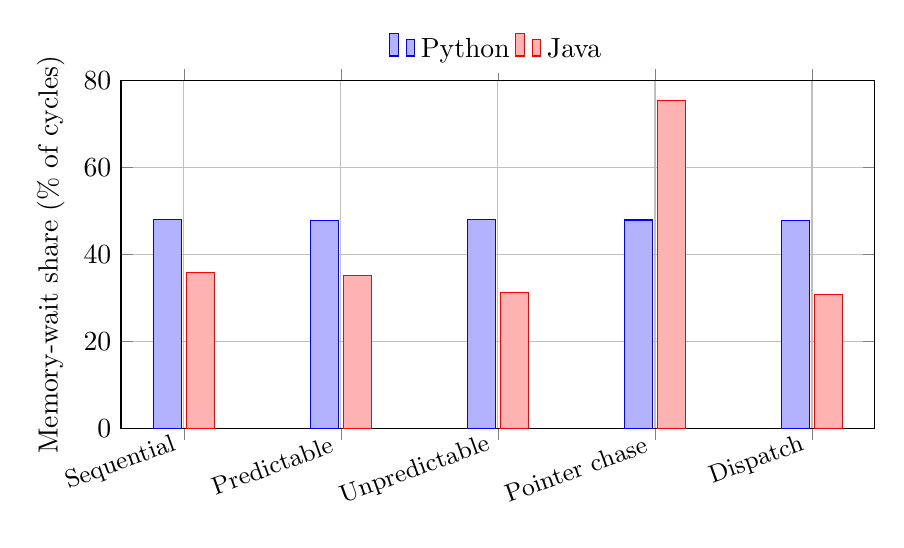
\begin{tikzpicture}
\begin{axis}[
  width=0.92\textwidth,
  height=6cm,
  ybar,
  bar width=10pt,
  symbolic x coords={Sequential,BranchPredictable,BranchUnpredictable,PointerChase,DynamicDispatch},
  xtick=data,
  xticklabels={Sequential,Predictable,Unpredictable,Pointer chase,Dispatch},
  x tick label style={rotate=20,anchor=east,font=\small},
  ylabel={Memory-wait share (\% of cycles)},
  ymin=0, ymax=80,
  ytick={0,20,40,60,80},
  grid=major,
  legend style={at={(0.5,1.02)},anchor=south,legend columns=2,draw=none},
]
\addplot coordinates {(Sequential,48.11) (BranchPredictable,47.89) (BranchUnpredictable,48.17) (PointerChase,47.96) (DynamicDispatch,47.75)};
\addplot coordinates {(Sequential,35.83) (BranchPredictable,35.29) (BranchUnpredictable,31.28) (PointerChase,75.46) (DynamicDispatch,30.93)};
\legend{Python,Java}
\end{axis}
\end{tikzpicture}
\caption{Memory-wait share by workload, using the simulator rule described in the text.}
\label{fig:memory-wait}
\end{figure}

\noindent\resizebox{\textwidth}{!}{%
\begin{tabular}{llrrrrrrrrr}
\toprule
Runtime & Workload & IPC & Branch MPKI & Conditional MPKI & Indirect-call MPKI & Accuracy (\%) & L1D miss (\%) & L1D latency & LLC miss (\%) & LLC latency \\
\midrule
Python & Sequential & 0.9716 & 12.490 & 11.800 & 0.009 & 94.79 & 4.44 & 172.8 & 99.65 & 180.9 \\
Python & BranchPredictable & 0.9921 & 12.340 & 11.670 & 0.007 & 94.86 & 4.49 & 171.4 & 98.56 & 180.8 \\
Python & BranchUnpredictable & 0.9801 & 12.570 & 11.890 & 0.006 & 94.77 & 4.43 & 172.4 & 99.72 & 181.0 \\
Python & PointerChase & 0.9899 & 12.430 & 11.760 & 0.006 & 94.82 & 4.39 & 173.2 & 99.28 & 178.8 \\
Python & DynamicDispatch & 0.9874 & 12.520 & 11.840 & 0.006 & 94.79 & 4.43 & 173.2 & 99.75 & 180.8 \\
Java & Sequential & 1.5000 & 20.470 & 0.220 & 0.000 & 90.18 & 0.83 & 179.0 & 100.00 & 154.3 \\
Java & BranchPredictable & 1.6170 & 8.271 & 7.863 & 0.000 & 96.43 & 0.04 & 210.3 & 100.00 & 185.0 \\
Java & BranchUnpredictable & 1.5290 & 23.520 & 6.027 & 0.000 & 89.88 & 0.00 & -- & 0.00 & -- \\
Java & PointerChase & 0.8578 & 0.219 & 0.219 & 0.000 & 99.90 & 2.04 & 154.7 & 100.00 & 171.6 \\
Java & DynamicDispatch & 1.4960 & 9.406 & 0.496 & 0.007 & 94.93 & 0.13 & 206.4 & 100.00 & 181.1 \\
\bottomrule
\end{tabular}%
}


\subsection{Retirement-stall classification}
ChampSim does not assign every lost cycle to one cause. I use a specific rule
to group zero-retirement cycles. This means cycles when no instruction retires.
If the reorder-buffer head waits on an issued load, I count it as
\emph{memory-wait}. Otherwise, I count it as \emph{pipeline/other}. These
groups do not overlap and add up to all zero-retirement cycles. Percentages
use total measured cycles. They do not include cycles with partial retirement.
This rule describes this simulator only. It is not a full hardware stall
breakdown.

\noindent\resizebox{\textwidth}{!}{%
\begin{tabular}{llrrr}
\toprule
Runtime & Workload & Zero-retire cycles (\%) & Memory-wait (\%) & Pipeline/other (\%) \\
\midrule
Python & Sequential & 66.79 & 48.11 & 18.68 \\
Python & BranchPredictable & 66.12 & 47.89 & 18.22 \\
Python & BranchUnpredictable & 66.39 & 48.17 & 18.22 \\
Python & PointerChase & 66.18 & 47.96 & 18.21 \\
Python & DynamicDispatch & 66.20 & 47.75 & 18.45 \\
Java & Sequential & 53.07 & 35.83 & 17.24 \\
Java & BranchPredictable & 47.96 & 35.29 & 12.67 \\
Java & BranchUnpredictable & 49.37 & 31.28 & 18.09 \\
Java & PointerChase & 78.60 & 75.46 & 3.13 \\
Java & DynamicDispatch & 52.87 & 30.93 & 21.95 \\
\bottomrule
\end{tabular}%
}


\subsection{Cache-capacity sensitivity}
I also tested caches with four times the baseline capacity. L1D grows from
48\,KiB to 192\,KiB. LLC grows from 2\,MiB to 8\,MiB. I changed one cache at a
time and kept all other settings. This checks sensitivity for these traces.
It does not isolate each cache's causal effect. Cache effects can overlap.

\noindent\resizebox{\textwidth}{!}{%
\begin{tabular}{lllrrrrr}
\toprule
Runtime & Workload & Configuration & IPC & Cycles & L1D miss (\%) & LLC miss (\%) & Cycle reduction (\%) \\
\midrule
Python & Sequential & Baseline & 0.9716 & 925240 & 4.44 & 99.65 & +0.00 \\
Python & Sequential & 4x L1D capacity & 0.9728 & 924125 & 4.09 & 99.84 & +0.12 \\
Python & Sequential & 4x LLC capacity & 0.9716 & 925240 & 4.44 & 99.65 & +0.00 \\
Python & BranchPredictable & Baseline & 0.9921 & 906208 & 4.49 & 98.56 & +0.00 \\
Python & BranchPredictable & 4x L1D capacity & 0.9947 & 903808 & 4.12 & 99.64 & +0.26 \\
Python & BranchPredictable & 4x LLC capacity & 0.9921 & 906208 & 4.49 & 98.56 & +0.00 \\
Python & BranchUnpredictable & Baseline & 0.9801 & 917252 & 4.43 & 99.72 & +0.00 \\
Python & BranchUnpredictable & 4x L1D capacity & 0.9848 & 912892 & 4.08 & 99.94 & +0.48 \\
Python & BranchUnpredictable & 4x LLC capacity & 0.9801 & 917252 & 4.43 & 99.72 & +0.00 \\
Python & PointerChase & Baseline & 0.9899 & 908178 & 4.39 & 99.28 & +0.00 \\
Python & PointerChase & 4x L1D capacity & 0.9913 & 906926 & 4.08 & 99.44 & +0.14 \\
Python & PointerChase & 4x LLC capacity & 0.9899 & 908178 & 4.39 & 99.28 & +0.00 \\
Python & DynamicDispatch & Baseline & 0.9874 & 910447 & 4.43 & 99.75 & +0.00 \\
Python & DynamicDispatch & 4x L1D capacity & 0.9906 & 907538 & 4.09 & 99.83 & +0.32 \\
Python & DynamicDispatch & 4x LLC capacity & 0.9874 & 910447 & 4.43 & 99.75 & +0.00 \\
Java & Sequential & Baseline & 1.5000 & 599312 & 0.83 & 100.00 & +0.00 \\
Java & Sequential & 4x L1D capacity & 1.5000 & 599312 & 0.83 & 100.00 & +0.00 \\
Java & Sequential & 4x LLC capacity & 1.5000 & 599312 & 0.83 & 100.00 & +0.00 \\
Java & BranchPredictable & Baseline & 1.6170 & 556029 & 0.04 & 100.00 & +0.00 \\
Java & BranchPredictable & 4x L1D capacity & 1.6170 & 556029 & 0.04 & 100.00 & +0.00 \\
Java & BranchPredictable & 4x LLC capacity & 1.6170 & 556029 & 0.04 & 100.00 & +0.00 \\
Java & BranchUnpredictable & Baseline & 1.5290 & 587846 & 0.00 & 0.00 & +0.00 \\
Java & BranchUnpredictable & 4x L1D capacity & 1.5290 & 587846 & 0.00 & 0.00 & +0.00 \\
Java & BranchUnpredictable & 4x LLC capacity & 1.5290 & 587846 & 0.00 & 0.00 & +0.00 \\
Java & PointerChase & Baseline & 0.8578 & 1048083 & 2.04 & 100.00 & +0.00 \\
Java & PointerChase & 4x L1D capacity & 0.8577 & 1048195 & 1.98 & 100.00 & -0.01 \\
Java & PointerChase & 4x LLC capacity & 0.8578 & 1048083 & 2.04 & 100.00 & +0.00 \\
Java & DynamicDispatch & Baseline & 1.4960 & 600818 & 0.13 & 100.00 & +0.00 \\
Java & DynamicDispatch & 4x L1D capacity & 1.4960 & 600818 & 0.13 & 100.00 & +0.00 \\
Java & DynamicDispatch & 4x LLC capacity & 1.4960 & 600818 & 0.13 & 100.00 & +0.00 \\
\bottomrule
\end{tabular}%
}
\par\medskip
\noindent Python: the largest cycle reduction across these workloads under either 4$\times$ capacity change was 0.48\%. These tests do not identify a cache-capacity level as dominant.\\
\noindent Java: the largest cycle reduction across these workloads under either 4$\times$ capacity change was 0.00\%. These tests do not identify a cache-capacity level as dominant.\\

\begin{figure}[htbp]
\centering
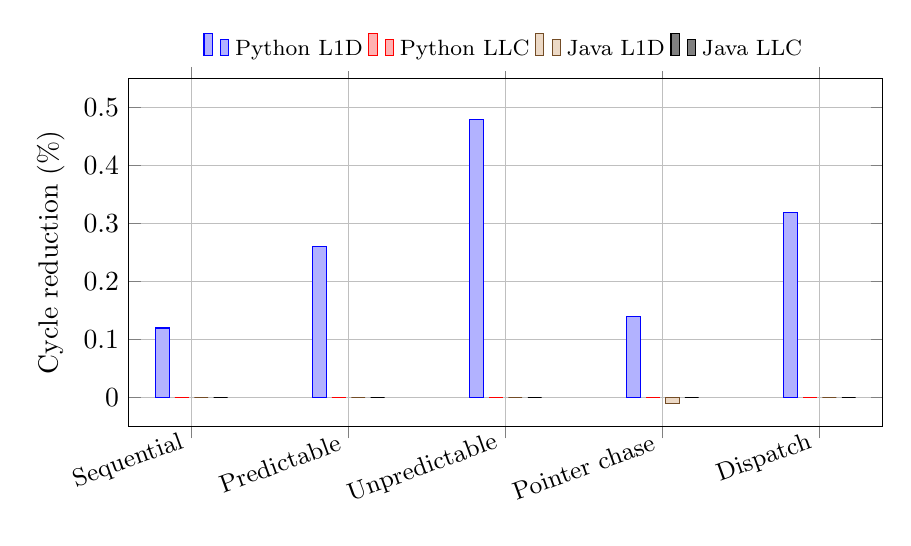
\begin{tikzpicture}
\begin{axis}[
  width=0.92\textwidth,
  height=6cm,
  ybar,
  bar width=5pt,
  symbolic x coords={Sequential,BranchPredictable,BranchUnpredictable,PointerChase,DynamicDispatch},
  xtick=data,
  xticklabels={Sequential,Predictable,Unpredictable,Pointer chase,Dispatch},
  x tick label style={rotate=20,anchor=east,font=\small},
  ylabel={Cycle reduction (\%)},
  ymin=-0.05, ymax=0.55,
  ytick={0,0.1,0.2,0.3,0.4,0.5},
  grid=major,
  legend style={at={(0.5,1.02)},anchor=south,legend columns=4,draw=none,font=\footnotesize},
]
\addplot coordinates {(Sequential,0.12) (BranchPredictable,0.26) (BranchUnpredictable,0.48) (PointerChase,0.14) (DynamicDispatch,0.32)};
\addplot coordinates {(Sequential,0.00) (BranchPredictable,0.00) (BranchUnpredictable,0.00) (PointerChase,0.00) (DynamicDispatch,0.00)};
\addplot coordinates {(Sequential,0.00) (BranchPredictable,0.00) (BranchUnpredictable,0.00) (PointerChase,-0.01) (DynamicDispatch,0.00)};
\addplot coordinates {(Sequential,0.00) (BranchPredictable,0.00) (BranchUnpredictable,0.00) (PointerChase,0.00) (DynamicDispatch,0.00)};
\legend{Python L1D,Python LLC,Java L1D,Java LLC}
\end{axis}
\end{tikzpicture}
\caption{Cycle reduction after increasing one cache's capacity by four times. Positive values mean fewer cycles.}
\label{fig:cache-sensitivity}
\end{figure}


\subsection{Paired workload contrasts}
These comparisons show how each pair differs in the measured traces. They do
not directly measure cycles lost to one source-level operation.
\textbf{Python branch-pattern contrast.} The unpredictable-pattern trace has +0.230 branch MPKI and -0.0120 IPC relative to the predictable-pattern trace. This is a trace-level contrast, not a direct count of cycles lost to branch mispredictions.

\textbf{Python memory-pattern contrast.} The pointer-chase trace differs from sequential access by -0.04 percentage points in L1D miss rate and -0.37 percentage points in LLC miss rate. Dependent-load latency is not equivalent to total memory-stall cycles.

\textbf{Java branch-pattern contrast.} The unpredictable-pattern trace has +15.249 branch MPKI and -0.0880 IPC relative to the predictable-pattern trace. This is a trace-level contrast, not a direct count of cycles lost to branch mispredictions.

\textbf{Java memory-pattern contrast.} The pointer-chase trace differs from sequential access by +1.22 percentage points in L1D miss rate and +0.00 percentage points in LLC miss rate. Dependent-load latency is not equivalent to total memory-stall cycles.


\section{Interpretation and limitations}
\subsection{What the patterns may mean}
Python's five workloads look similar in these traces. IPC ranges from 0.9716
to 0.9921. L1D miss rates stay near 4.4\%. Pointer chasing does not have a
higher miss rate than sequential access here. Interpreter instructions may
hide differences between the workloads. The pointer pattern may also fit the
measured caches better than expected. These results cannot tell which
explanation is correct.

Java pointer chasing stands out. It has the lowest IPC, at 0.8578. Its
memory-wait share is 75.46\%, compared with 35.83\% for sequential access.
Each pointer load depends on the previous load. This may leave fewer
independent memory requests while the processor waits. The measurements fit
this explanation, but do not prove it. Pointer chasing has a 2.04\% L1D miss
rate, and all its LLC accesses miss. These numbers need to be read together.

The Java branch results also need care. Unpredictable branching has 15.249
more total branch MPKI than predictable branching. But its conditional-branch
MPKI is lower. Indirect-branch MPKI rises from 0.246 to 17.500. PIN records
native instructions, not just branches in the source code. So this difference
may include runtime control flow. It would be wrong to blame it all on the
benchmark's conditional. Python's total branch MPKI changes less, by 0.230.

Larger caches made little difference to cycle counts. A larger L1D reduced
Python's miss rate slightly. Its largest cycle reduction was 0.48\%. A larger
LLC did not reduce cycles in these runs. The tests cannot show whether misses
were hidden by other work or were not helped by extra capacity. They do not
show that cache misses are unimportant in general.

\subsection{Limits of these results}
Each result comes from one 1,000,000-instruction trace window. I did not
measure variation across repeat runs. Longer traces and repeat runs could show
whether these patterns last. Java traces exclude JVM background threads and
use PIN-specific launch options. They may not match a default production JVM.
The stall groups use the rule described above. They are not a complete
hardware stall breakdown. This report cannot identify one general bottleneck
for either language.

\subsection{Takeaway}
For these traces, Java pointer chasing was the clearest outlier. Python's
workloads looked similar. Larger caches barely changed cycle counts. The
results answer the initial question only for these short traces. Next, I
would repeat the runs and use longer trace windows.

\section{Reproducibility}
Run \texttt{make checkpoint1} from the project root. Override
the trace-skip, trace-length, warmup, and simulation-length settings to choose
the capture and measurement region. Reproduce the settings used for these
results and regenerate the metrics table/CSV with:
\begin{verbatim}
make checkpoint1 TRACE_SKIP_INSTRUCTIONS=5000000 \
  TRACE_INSTRUCTIONS=1000000 WARMUP_INSTRUCTIONS=100000 \
  SIMULATION_INSTRUCTIONS=899000
python3 analysis/summarize_checkpoint1.py \
  --trace-skip 5000000 --trace-instructions 1000000 \
  --simulation-instructions 899000
python3 analysis/summarize_cache_sensitivity.py
\end{verbatim}
These commands also generate the plot files included in the report.
Compile this report with:
\begin{verbatim}
pdflatex checkpoint1_report.tex
\end{verbatim}
The detailed metrics are also saved in \texttt{checkpoint1\_metrics.csv}.

\end{document}
